\section{The Web Application}

To complement the \ac{CLI},
we developed a web application
to provide a user-friendly interface for running the whole end-to-end pipeline,
that is, to run \ac{TRACER} to generate the user profiles,
and then to execute these with SENSEI.
This, enables a broader audience to use both \ac{TRACER} and SENSEI
without the need of knowing how to use the \ac{CLI}.

\subsection{System Architecture}

The web application is built on a modern,
multi-tiered architecture designed for scalability, security, and asynchronous processing.
\autoref{fig:app-architecture} provides an overview of this architecture,
illustrating the relationships between the five key layers:
the Client, Presentation, Application, Task Processing, and Data layers.
The following subsections will provide a detailed explanation
of the technologies and design patterns used within each of these layers.

\begin{figure}[!htbp]
    \centering
    \begin{tikzpicture}[
    auto,
    node distance=1.3cm and 1cm,
    every node/.style={align=center},
    rect_node/.style={rectangle, draw, thick, rounded corners=3pt},
    client/.style={rect_node, fill=blue!20, minimum height=1.5em, minimum width=6em},
    proxy/.style={rect_node, fill=orange!20, minimum height=2em, minimum width=7em},
    frontend/.style={rect_node, fill=green!20, minimum height=2em, minimum width=6em},
    backend/.style={rect_node, fill=yellow!20, minimum height=2.5em, minimum width=7em},
    worker/.style={rect_node, fill=cyan!20, minimum height=1.5em, minimum width=6em},
    broker/.style={rect_node, fill=pink!20, minimum height=2em, minimum width=6em},
    analysis/.style={rect_node, fill=red!20, minimum height=1.5em, minimum width=4.5em},
    storage/.style={rect_node, fill=purple!20, minimum height=2em, minimum width=5em},
    db/.style={cylinder, shape border rotate=90, draw, fill=blue!20, aspect=0.4, minimum height=2.5em, minimum width=5em},
    layer/.style={rectangle, fill=gray!10, rounded corners},
    arrow/.style={-Stealth, thick},
    async_arrow/.style={-Stealth, thick, dashed, red},
    data_arrow/.style={-Stealth, thick, blue},
    label_bg/.style={fill=white, inner sep=2pt, rounded corners=8pt},
    layer_label/.style={font=\small\bfseries, rounded corners=3pt, inner sep=3pt, fill=white}
]

    % NODES
    \node[client] (user) {User Browser};
    \node[proxy, below=of user, yshift=-0.5cm] (nginx) {Nginx Proxy\\Port 80};
    \node[frontend, right=of nginx, xshift=1.5cm] (react) {React SPA\\(Build Files)};
    \node[backend, below=of nginx, yshift=-1.5cm] (django) {Django App\\REST API\\Port 8000};
    \node[db, right=of django, xshift=2cm] (postgres) {PostgreSQL\\Port 5432};
    \node[broker, left=of django, xshift=-2cm] (rabbitmq) {RabbitMQ\\Broker\\Port 5672};
    
    \node[worker, below=of rabbitmq] (celery) {Celery Worker};
    \node[analysis, below=of celery, xshift=-1.2cm] (tracer) {TRACER};
    \node[analysis, below=of celery, xshift=1.2cm] (sensei) {Sensei};
    \node[storage, below=of postgres, yshift=-0.2cm] (filevault) {File Vault};
    \node[storage, below=of filevault, yshift=-0.2cm] (staticfiles) {Django Static\\Files};

    % BACKGROUNDS
    \begin{scope}[on background layer]
        \node[layer, fit=(user)] (user_layer) {};
        \node[layer, fit=(nginx)(react)] (presentation_layer) {};
        \node[layer, fit=(django)] (application_layer) {};
        \node[layer, fit=(rabbitmq)(celery)(tracer)(sensei)] (task_layer) {};
        \node[layer, fit=(postgres)(filevault)(staticfiles)] (data_layer) {};
    \end{scope}

    % CONNECTIONS
    \draw[arrow] (user) -- node[label_bg, left, pos=0.5] {HTTP} (nginx);
    \draw[arrow] (nginx) -- node[above] {Serves SPA} (react);
    \draw[arrow] (nginx) -- node[label_bg, left, pos=0.35, align=right] {/api/\\/admin/\\/filevault/} (django);
    \draw[arrow] (react.south) to[bend right=20] node[label_bg, right, pos=0.5] {REST API\\Calls} (django.north east);
    \draw[arrow] (nginx.east) to[out=-45, in=125] node[label_bg, below, pos=0.1] {/static/} (staticfiles.north west);
    \draw[data_arrow] (django.east) to[bend left=15] node[above, pos=0.25] {queries} (postgres.west);
    \draw[data_arrow] (django.east) to[out=-60, in=200, looseness=0.9] node[left, pos=0.6] {file\\operations} (filevault.west);
    \draw[async_arrow] (django.west) -- node[label_bg, above] {queue} (rabbitmq.east);
    \draw[async_arrow] (rabbitmq) -- node[right] {consume} (celery);
    \draw[async_arrow] (celery) -- node[left] {execute} (tracer);
    \draw[async_arrow] (celery) -- node[right] {execute} (sensei); 
    \draw[async_arrow] (celery.east) to[bend right=20] node[above, pos=0.25] {task results\\and status} (postgres.west);
    \draw[data_arrow] (celery.east) to[bend right=45] node[below, pos=0.5] {file\\operations} (filevault.west);

    % FOREGROUND LAYER LABELS 
    \node[layer_label, yshift=0.5cm] at (user_layer.north) {Client Layer};
    \node[layer_label, yshift=0.5cm] at (presentation_layer.north) {Presentation Layer};
    \node[layer_label, yshift=0.5cm] at (application_layer.north) {Application Layer};
    \node[layer_label, yshift=0.5cm] at (task_layer.north) {Task Processing Layer};
    \node[layer_label, yshift=0.5cm] at (data_layer.north) {Data Layer};

    % Legend
    \node[anchor=north west, align=left, yshift=0.5cm] at (current bounding box.south west) {
        \begin{tabular}{@{}ll}
            \multicolumn{2}{l}{\textbf{Legend:}}\\
            \tikz{\draw[arrow] (0,0.5ex) -- (0.5,0.5ex);} & HTTP Flow\\
            \tikz{\draw[async_arrow] (0,0.5ex) -- (0.5,0.5ex);} & Async Tasks\\
            \tikz{\draw[data_arrow] (0,0.5ex) -- (0.5,0.5ex);} & Data Access
        \end{tabular}
    };
\end{tikzpicture}

    \caption{Web Application Architecture and Connections.}
    \label{fig:app-architecture}
\end{figure}

\subsection{Core Technology Stack}

The backend of the application was developed in Django \autocite{Django},
This framework was chosen because it is Python-based
and therefore compatible with \ac{TRACER} and SENSEI,
and also it offers the Django REST Framework \autocite{DjangoRESTFramework}
which enables the development of a \ac{REST} \ac{API}
that will be consumed by our frontend.

For the frontend we chose React \autocite{React},
a JavaScript library to develop \acp{SPA}
which consumes data directly from our Django \ac{API}.

Lastly, to ensure data persistence,
we used PostgreSQL \autocite{PostgreSQL2025},
we chose a \ac{SQL} database since Django's \ac{ORM} supports this type of databases out of the box,
also, we preferred PostgreSQL over the default Django's SQLite
since the latter is more oriented to development and testing
and stores everything in a single file which causes concurrency and performance issues when used in production.

\subsection{Asynchronous Task Handling}

\ac{TRACER} and SENSEI executions both take from a few minutes up to hours,
thus, executing this tasks synchronously would leave the user's interface unresponsive
for the duration of the whole process.
To handle this we implemented asynchronous executions,
we did this by using a distributed task queue called Celery \autocite{Celery},
which enables these jobs to be handled asynchronously.
Then, to communicate Django with Celery we need a broker,
for this we used RabbitMQ \autocite{RabbitMQ}.
These two tools in conjunction will allow the user to execute \ac{TRACER} or SENSEI
and change to a different view, log out, or even turn off the computer
and later return to check its progress.
It will also prevent server overload
since we can limit the number of concurrent jobs
and if there are requests to execute more than this number,
the jobs will be waiting on the queue instead of saturating the server.


\subsection{The Nginx Reverse Proxy}

\begin{figure}[htbp]
    \centering
    \begin{tikzpicture}[
    node distance=1cm and 0.8cm, 
    box/.style={rectangle, draw, thick, text centered, minimum height=1.2cm, minimum width=2.8cm, align=center, rounded corners=3pt},
    arrow/.style={-Stealth, thick},
    label_bg/.style={fill=white, inner sep=1.5pt, rounded corners=3pt}
]
    \node[box, fill=blue!20] (client) {Client Browser\\Port 80};
    \node[box, fill=orange!20, below=1.2cm of client] (nginx) {Nginx Proxy\\Port 8080};

    \node[box, fill=green!20, below left=of nginx] (react) {React Files\\/var/www/react};
    \node[box, fill=purple!20, below=2cm of nginx] (static) {Static Files\\/var/www/static};
    \node[box, fill=yellow!20, below right=of nginx] (backend) {Django API\\backend:8000};

    \draw[arrow] (client) -- (nginx);
    \draw[arrow] (nginx) -- node[label_bg, above left, font=\footnotesize] {/} (react);
    \draw[arrow] (nginx) -- node[label_bg, right, font=\footnotesize] {/static/} (static);
    
    \draw[arrow] (nginx) -- node[label_bg, above right, font=\footnotesize, align=right] {/api/, /admin/,\\/filevault/} (backend);

\end{tikzpicture}

    \caption{Nginx routing to serve React, Django's static files and Django API.}
    \label{fig:nginx-routing}
\end{figure}

A reverse proxy is essential for managing the communication between
the user, the React frontend, and the Django backend.
For this role, we used Nginx \autocite{Nginx}.
Its primary responsibility is to route incoming HTTP requests to the appropriate service based on the URL path.
This also addresses the challenge of accessing each service in a different port,
although they are running in a different port
we can always access the same URL and Nginx will redirect the call.

In the \autoref{fig:nginx-routing}
we can see the configuration of the reverse proxy.
It recieves all the calls from the users and routes them to the correct service.
We have that all calls made to \texttt{/api/}, \texttt{/admin/} and \texttt{/filevault/}
get redirected to Django's backend since as it processes \ac{API} calls,
return the different files and show the admin dashboard.
The Django admin dashboard requires its CSS to be rendered correctly,
which in turn necessitates serving the Django static files.
For this reason, any request made to the \texttt{/static/} path
is redirected to the location of these files.
Lastly, the remaining calls will be redirected to React's build files.

\subsection{Deployment and Containerisation}



To facilitate the deployment of these services
we containerized the whole web application using Docker \autocite{merkelDockerLightweightLinux2014} along Docker compose.
This was done not only to simplify the deployment process,
but to ensure that no matter the machine and the dependencies it had installed,
it would work if it had Docker.
We made two different Docker compose versions, one for development and one for production,
each with their own \ac{DB}, message broker, and so on.
So that production data was not affected during development.
The complete production architecture is shown in \autoref{fig:docker-architecture}.

\begin{figure}[htpb]
    \centering
    \begin{tikzpicture}[
    node distance=0.4cm and 1.5cm,
    container/.style={rectangle, draw, thick, text centered, minimum height=1cm, minimum width=3.2cm, align=center, rounded corners=3pt},
    volume/.style={cylinder, shape border rotate=90, draw, fill=gray!20, text centered, minimum height=1.2cm, minimum width=2.2cm, aspect=0.3, align=center},
    dependency/.style={-Stealth, dashed, thick, red},
    mount/.style={-, thick, blue}
]
    % MIDDLE TIER: Application Containers (Central anchors)
    \node[container, fill=yellow!20] (backend) {Backend\\Django API\\Port 8000};
    \node[container, fill=green!20] (frontend) [left=of backend] {Frontend\\React Build};
    \node[container, fill=blue!20] (celery) [right=of backend] {Celery Worker\\Async Tasks};

    % BOTTOM TIER: Backing Services
    \node[container, fill=cyan!20] (db) [below=of backend, xshift=-2.8cm] {postgres:16\\Port 5432};
    \node[container, fill=pink!20] (rabbitmq) [below=of backend, xshift=2.8cm] {rabbitmq:3-mgmt\\Port 5672};
    
    % VOLUMES (placed relative to the structure)
    \node[volume] (staticfiles) [above=of backend] {static\_files\_prod};
    \node[volume] (reactbuild) [left=of staticfiles] {react\_build};
    \node[volume] (filevault) [right=of staticfiles] {filevault\_data\_prod};
    
    % TOP TIER: Nginx placed cleanly above the volumes
    \node[container, fill=orange!20] (nginx) [above=of staticfiles] {nginx:latest\\Port 80→8080};
    
    % Bottom row of volumes, dedicated to their services
    \node[volume] (pgdata) [below=of db] {postgres\_data};
    \node[volume] (rmqdata) [below=of rabbitmq] {rabbitmq\_data};

    % Dependency arrows (red dashed)
    \draw[dependency] (backend) -- (db);
    \draw[dependency] (backend) -- (rabbitmq);
    \draw[dependency] (celery) -- (db);
    \draw[dependency] (celery) -- (rabbitmq);
    \draw[dependency] (frontend) -- (backend);
    \draw[dependency] (nginx) -- (frontend);
    \draw[dependency] (nginx) to[bend left=70] (backend);

    % Volume mounts (blue solid)
    \draw[mount] (db.south) -- (pgdata.north);
    \draw[mount] (rabbitmq.south) -- (rmqdata.north);
    \draw[mount] (frontend.north) -- (reactbuild.south);
    \draw[mount] (backend.north) -- (staticfiles.south);
    \draw[mount] (celery.north) -- (filevault.south);
    \draw[mount] (nginx) to[bend left=10] (reactbuild);
    \draw[mount] (nginx) -- (staticfiles);
    \draw[mount] (backend) to[bend right=15] (filevault);
    \draw[mount] (celery) to[bend left=15] (staticfiles);

    % Legend anchored to the bottom-left of the picture
    \node[anchor=north west, align=left, yshift=-0.4cm] at (current bounding box.south west) {
        \begin{tabular}{@{}ll}
            \multicolumn{2}{l}{\textbf{Legend:}}\\
            \tikz{\draw[dependency] (0,0.5ex) -- (0.5,0.5ex);} & Container Dependency\\
            \tikz{\draw[mount] (0,0.5ex) -- (0.5,0.5ex);} & Volume Mount\\
        \end{tabular}
    };
\end{tikzpicture}

    \caption{Docker Container Architecture.}
    \label{fig:docker-architecture}
\end{figure}

In the \autoref{fig:docker-architecture} we show how the production containers and volumes are organized.
Each square is a container running said service,
then each cylinder is volume, where files are stored to ensure data persistance when containers are taken down.
Each blue arrow means that the volume is mounted in that container, i.e., the container can access the volume's files,
and the red ones show dependencies for the Docker compose,
which means that until the container that the arrow is pointing at is not working,
the container at the start of the arrow will not be initiated.

This ensures that until we do not have the \ac{DB} and message broker set
the queue and backend will not start,
and only then the frontend will be built
and lastly the Nginx reverse proxy.
In the development version the setup was mostly the same
but we had another volume that had the frontend and backend code
so that we would have hot reload (i.e., changes in the code were shown live in the web).

\subsection{Security Measures}

To ensure the application's security we followed the Django Deployment Checklist \autocite{DeploymentChecklistDjango}.
Related to the authentication we implemented a new user model,
and to handle the authentication we used Django-Rest-Knox \autocite{DjangoRestKnox} tokens.
This is a library that implements an improved token system over the default in the Django REST Framework \autocite{DjangoRESTFramework},
the main improvements include:
\begin{itemize}
  \item \textbf{One token per device:}
    instead of having one token per user
    which would mean that logging in from different devices
    would mean that they share the same token,
    causing that for example
    logging out on one device would terminate the session on all others.
    Knox solves this by creating one token per device.

  \item \textbf{Encrypted token in \ac{DB}:}
    this is a major security flaw from \ac{DRF}
    and it is that tokens are stored as plain text in the \ac{DB},
    meaning that if the \ac{DB} was compromised,
    the attacker could use those tokens to impersonate the legitimate user.

  \item \textbf{Token expire time:}
    in \ac{DRF}, once an account is authenticated, the generated token remains valid indefinitely.
    Knox, in contrast, allows an expiry time to be set.
    After this period, the session is terminated as the token becomes invalid.
\end{itemize}

To store the \ac{API} keys uploaded by the user to run \ac{TRACER} or SENSEI
we used Fernet Symmetric Encryption \autocite{FernetSymmetricEncryption}
to encrypt them before saving them to the \ac{DB}.
Although the \ac{DB} has a user and password (not the default ones)
we determined this was a prudent measure to add further layers of security,
the same way that Knox encrypts, so that
if the database was compromised, these credentials would remain encrypted.

These measures, combined with strict access controls,
ensure the application adheres to robust security practices.
Every request to the \ac{API} requires token validation.
Furthermore, models are configured to be readable only by their owner,
unless explicitly set to public.
Even when a project is public, write access remains restricted to the owner.


\subsection{User Workflow and Features}

This section aims to illustrate the web application,
describing the typical end-to-end workflow
a user follows within the web application.
The web application is available at \url{http://miso.ii.uam.es:8081/}.

\begin{figure}[htpb]
  \centering
  \makebox[\textwidth][c]{
    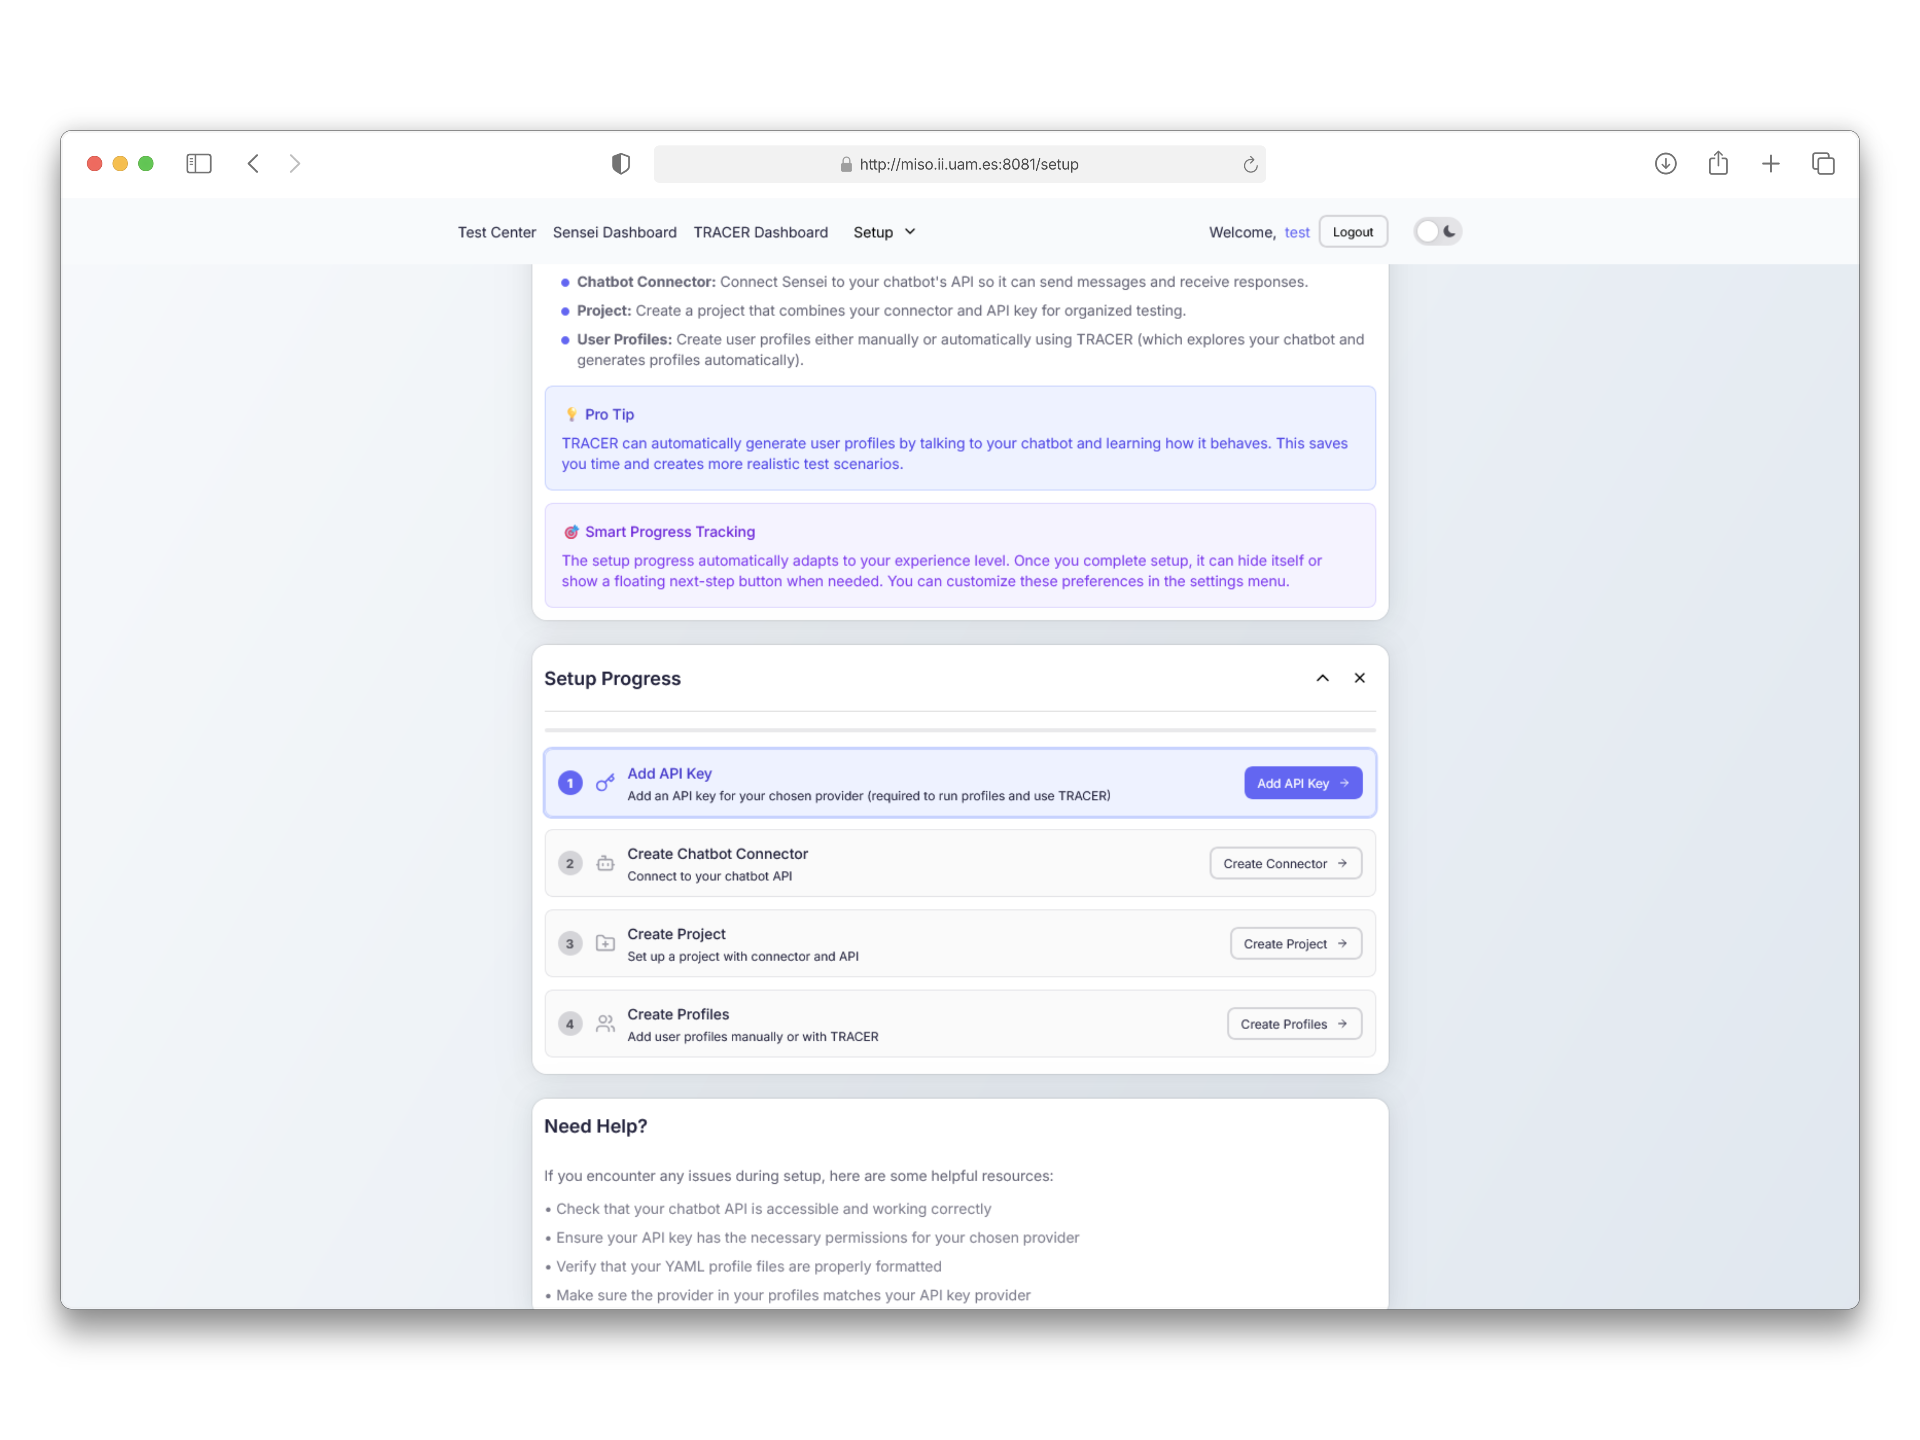
\includegraphics[width=1.1\textwidth]{figures/web-screenshots/setup-guide.png}
  }
  \caption{Screenshot of the setup guide.}
  \label{fig:ss-setup-guide}
\end{figure}

When users enter the web page
they are presented with an authentication page
that allows them to log in or register.
Once logged in,
the user is presented with the setup guide,
as shown in \autoref{fig:ss-setup-guide}.
This guide assists users in configuring the environment
before they can run \ac{TRACER} or SENSEI.
This guided tour is dynamic,
meaning that as the user completes steps
it automatically advances to the next step
and displays a button to navigate the user directly there.
The setup guide can also be closed,
and if required, there is a section in the navbar called "Setup Guide"
from which the user can open it again or read it in detail.

\begin{figure}[!htb]
  \centering
  \makebox[\textwidth][c]{
    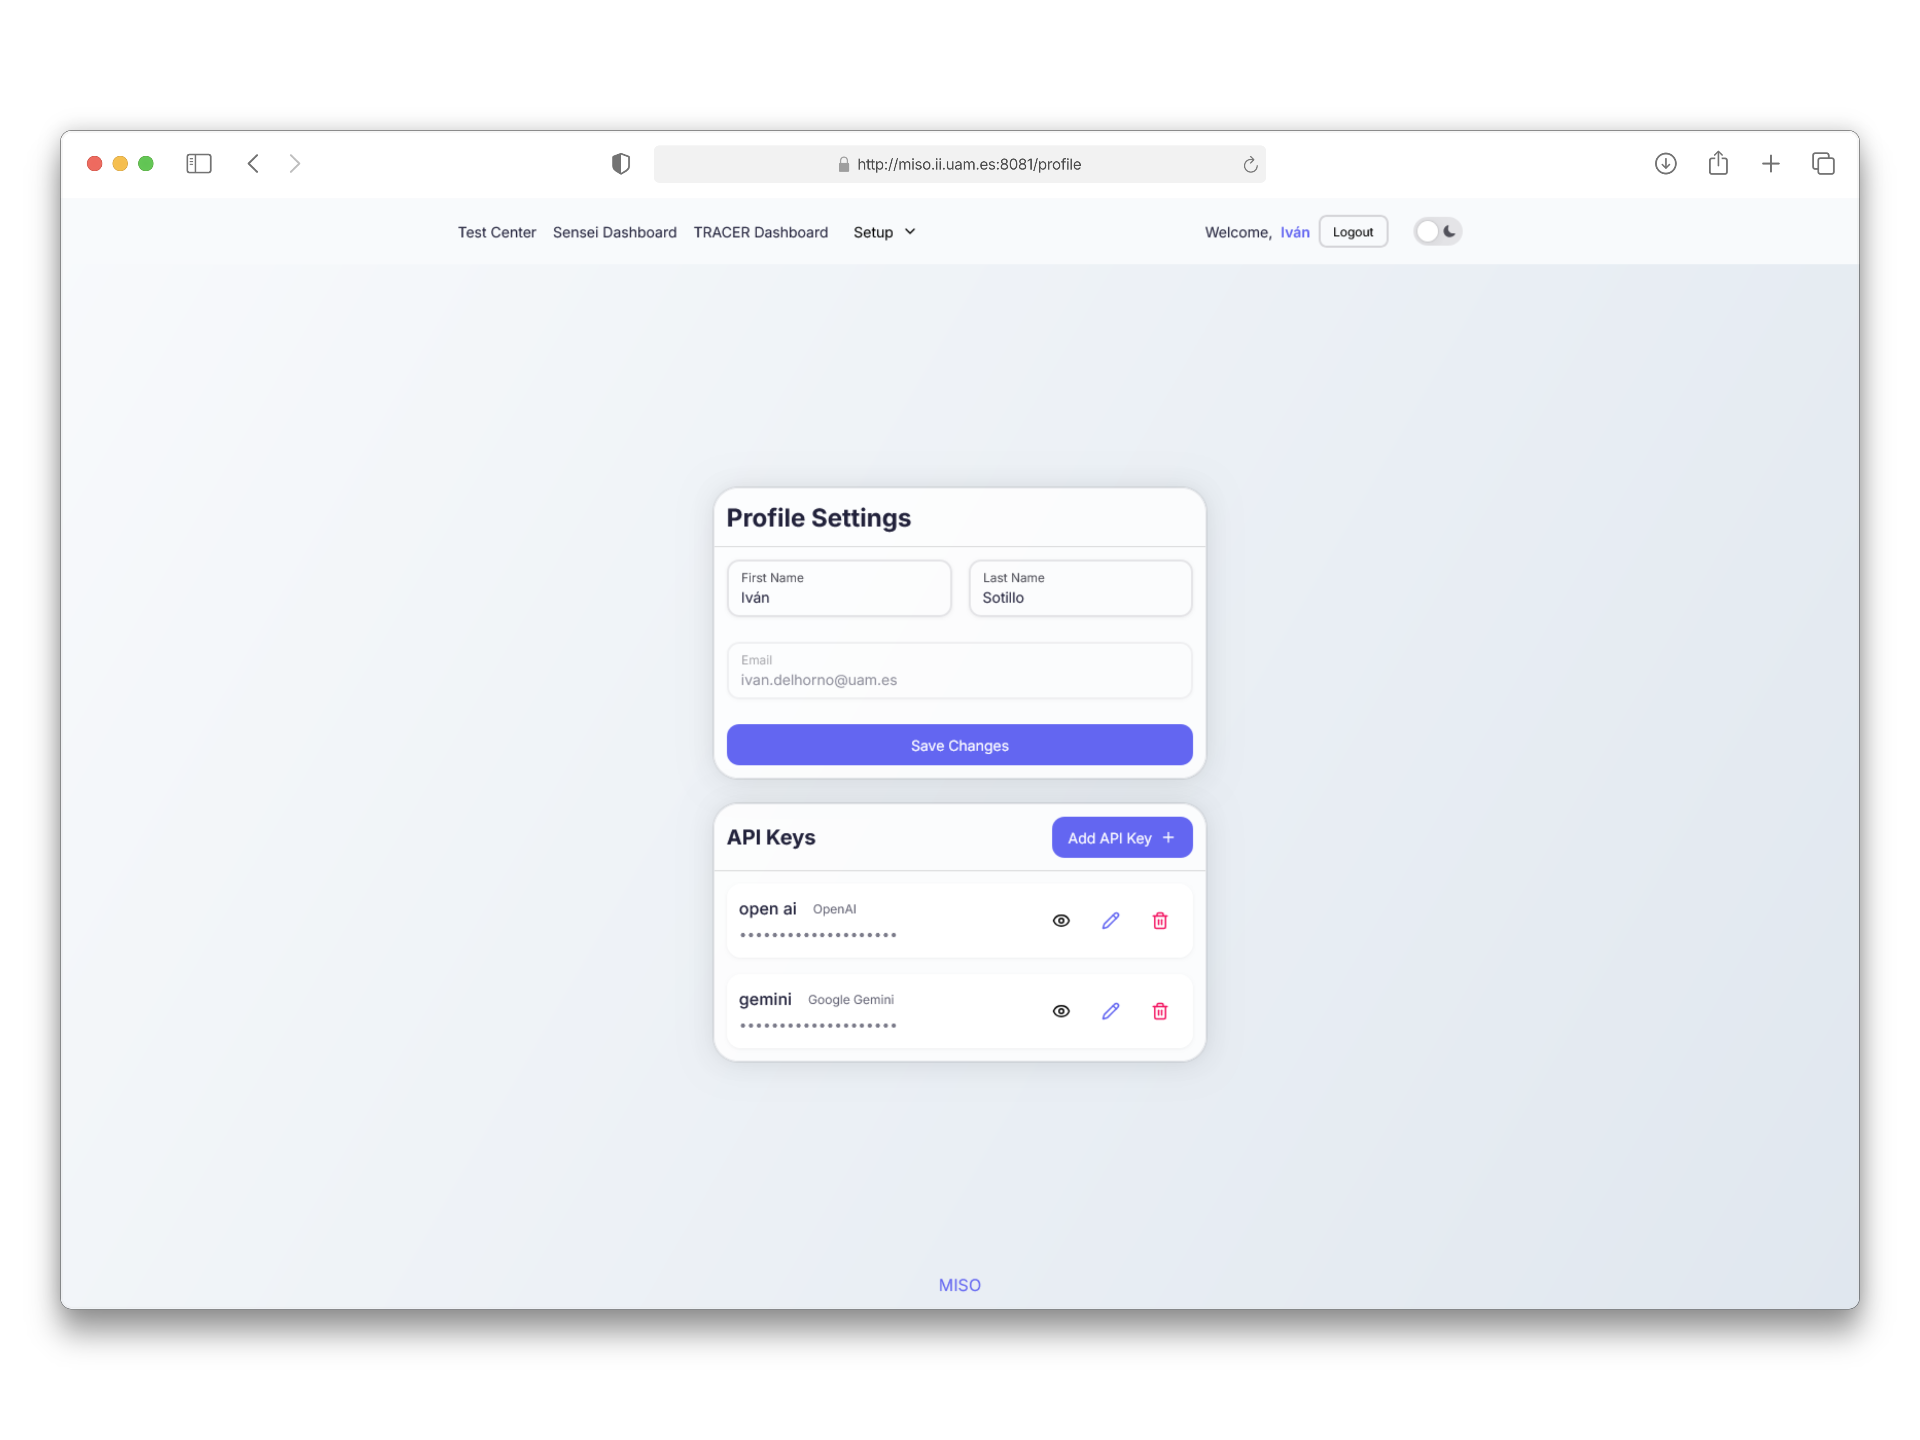
\includegraphics[width=1.1\textwidth]{figures/web-screenshots/profile.png}
  }
  \caption{Screenshot of the user profile view where users can set up their API key.}
  \label{fig:ss-profile}
\end{figure}

The first step in the guided setup
is to configure the necessary \ac{LLM} credentials.
As shown in \autoref{fig:ss-profile}
this is accomplished from the profile view.
A \ac{BYOK} approach was chosen,
that is, instead of charging per usage
each user brings their own \ac{API} key
therefore, they only pay for what they use.
The user can save OpenAI and Gemini \ac{API} keys.
These will be used both by \ac{TRACER} and SENSEI.

\begin{figure}[htpb]
  \centering
  \makebox[\textwidth][c]{
    \begin{subfigure}{0.52\textwidth}
      \centering
      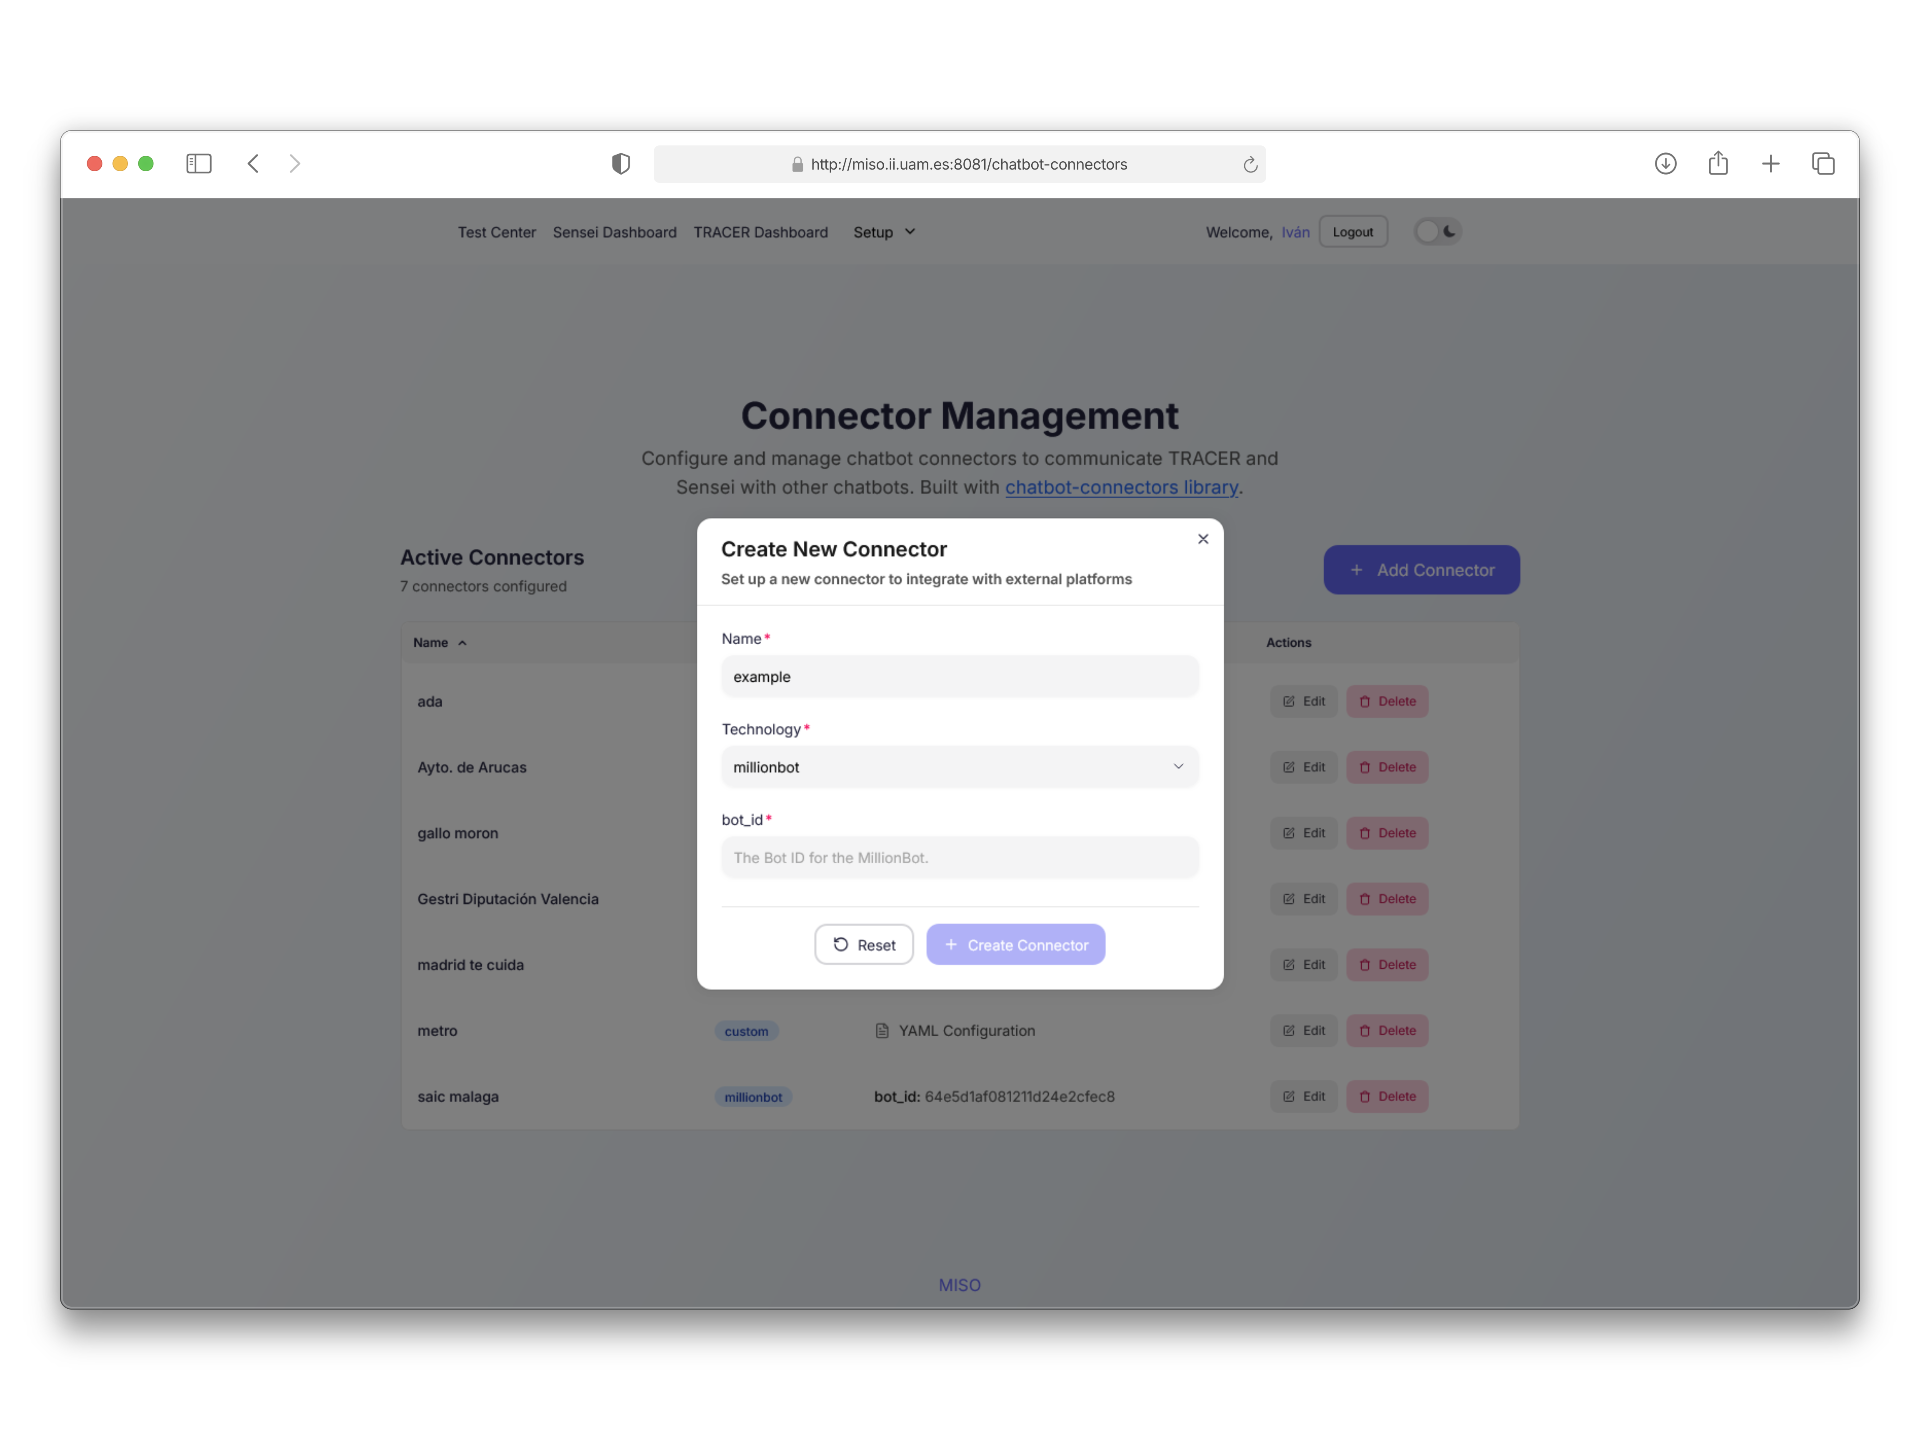
\includegraphics[width=\linewidth]{figures/web-screenshots/create-new-connector.png}
      \caption{Create new connector modal with the connectors dashboard behind it.}
      \label{fig:ss-new-connector}
    \end{subfigure}
    \begin{subfigure}{0.52\textwidth}
      \centering
      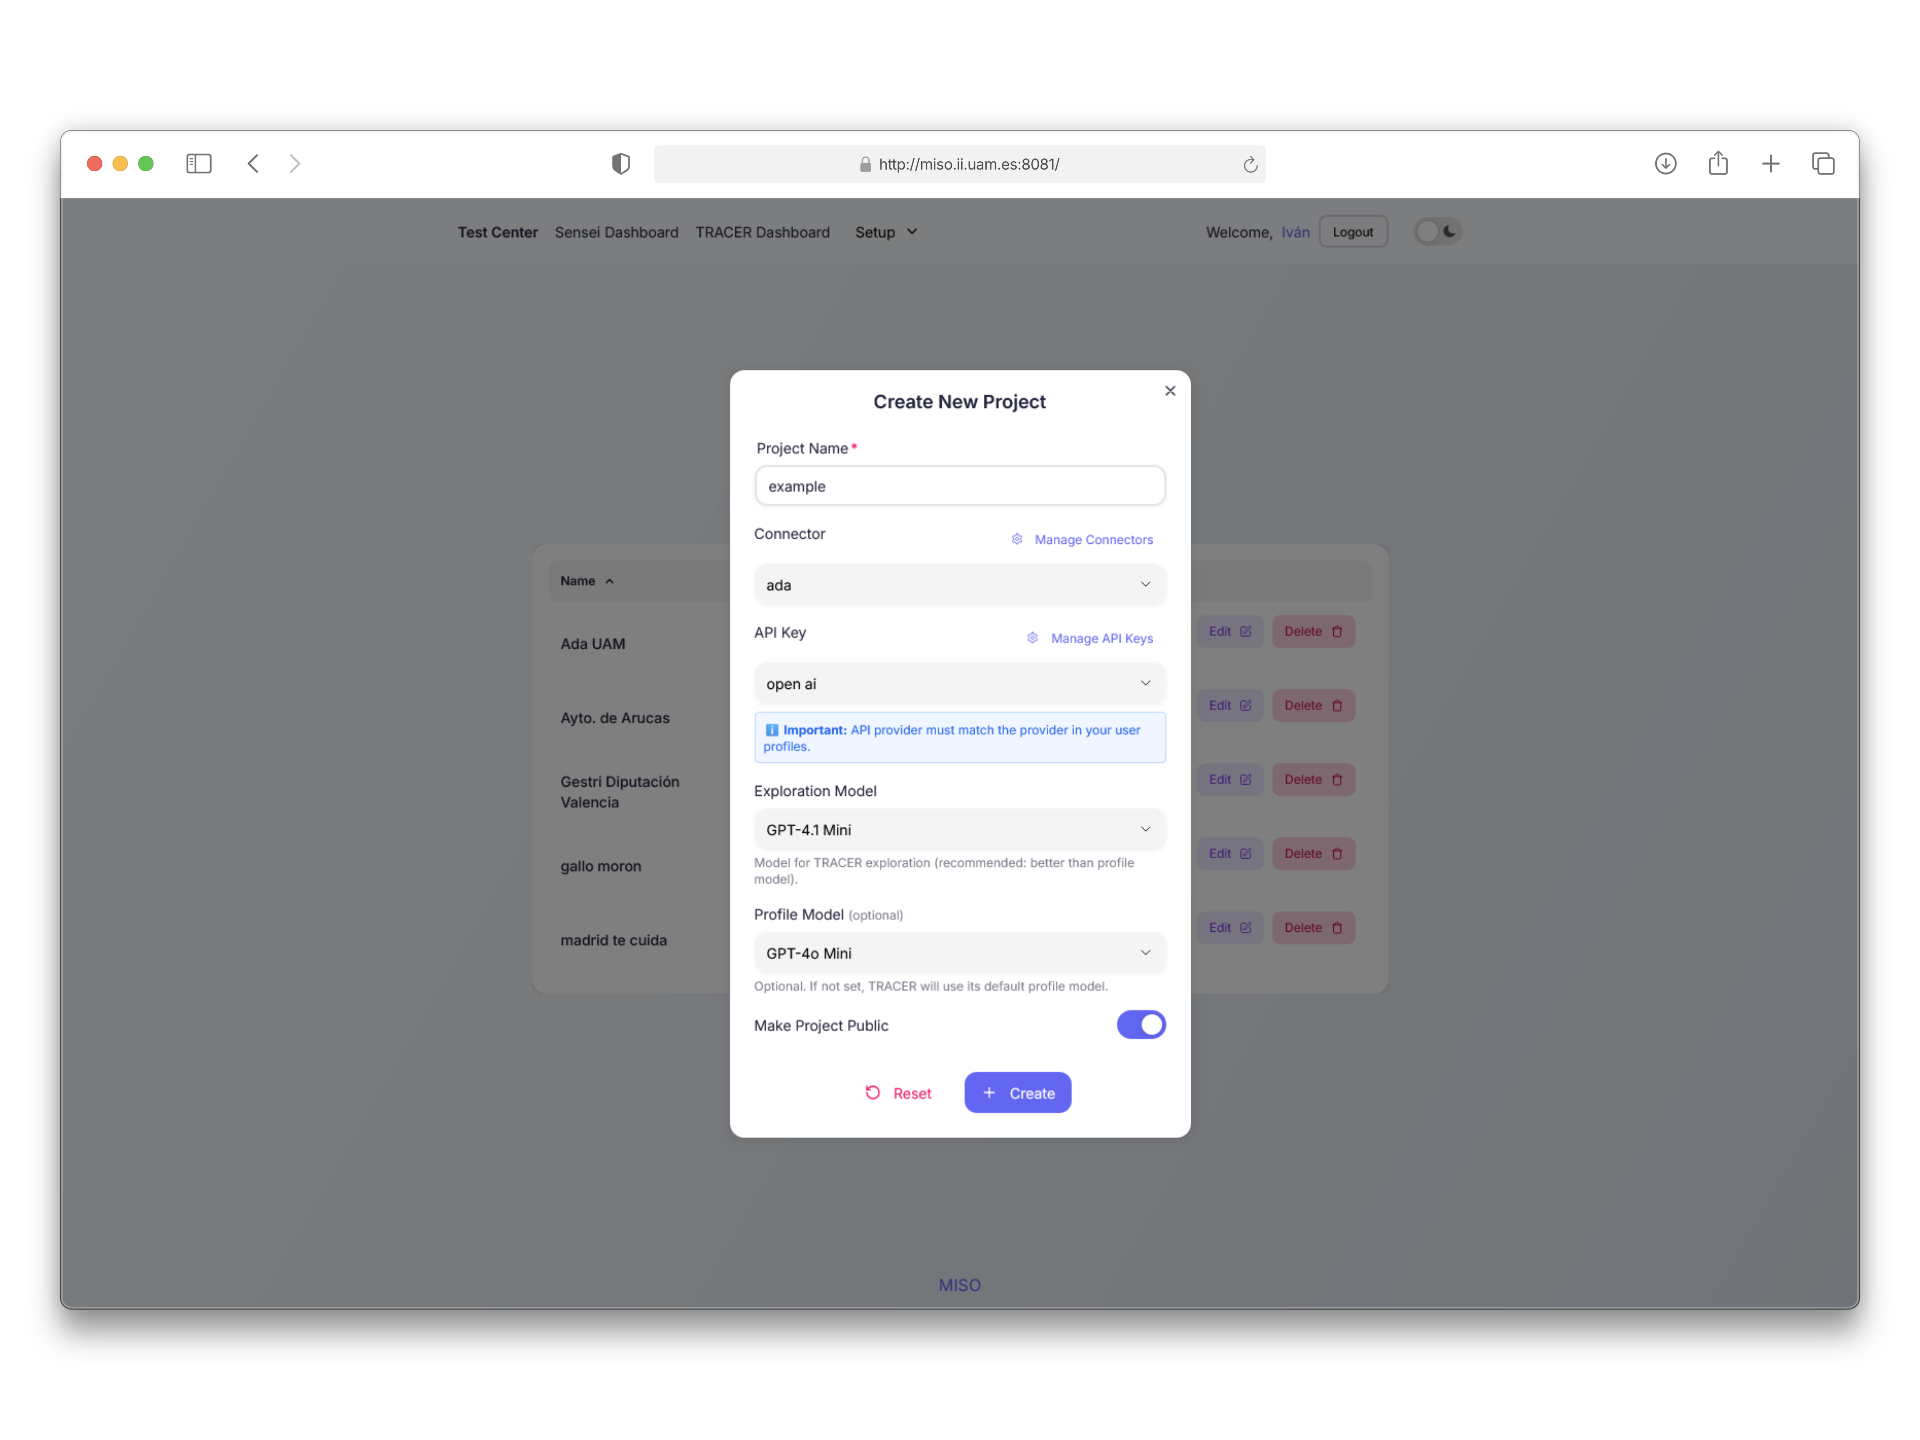
\includegraphics[width=\linewidth]{figures/web-screenshots/create-project-modal.png}
      \caption{Create new project modal with the project dashboard behind it.}
      \label{fig:ss-new-project}
    \end{subfigure}
  }
  \caption{Screenshots of the create new connector and create new project modals.}
  \label{fig:ss-modals}
\end{figure}

The next step is to define the chatbot connectors.
As explained in \autoref{sec:chatbot-connectors},
these are reusable configurations
that enable connection to chatbots via an \ac{API}.
There are two main methods for creating a connector:
\begin{itemize}
  \item \textbf{Built-in connectors:}
    for technologies that are already configured
    in the \texttt{chatbot-connectors} library,
    such as Taskyto, Rasa or MillionBot,
    the interface presents a dynamic form
    that prompts the user for the specific parameters
    required for that platform
    (e.g., a \texttt{bot\_id} for MillionBot,
    or \texttt{url} and \texttt{port} for Taskyto).
  \item \textbf{Custom YAML Connector:}
    for other chatbots that are not available in the list of options,
    but that offer a \ac{REST} \ac{API},
    the user can select the custom option.
    This option opens a YAML editor
    where the users declaratively define the connection.
    To facilitate this process, a set of helpful features was added to the editor,
    such as documentation and examples.
\end{itemize}


Once the \ac{API} keys and connectors are configured
the user is ready to create a project.
A project is the central workspace when working on a chatbot,
it will contain, in addition to the already mentioned \ac{API} key and connector,
the \ac{TRACER} and SENSEI executions.
To create a project the user must complete a form,
assigning it a name, selecting one of the connectors and \ac{API} keys
and also two \acp{LLM}, one for the exploration and another for the generated profiles,
the list of \acp{LLM} is dynamically updated based on the provider of the \ac{API} key.
Lastly, the users select whether the project should be public.
If a project is public, other users will be able to freely view the results
in the SENSEI and \ac{TRACER} dashboards.
This menu is shown in \autoref{fig:ss-new-project}.

\begin{figure}[!htb]
  \centering
  \makebox[\textwidth][c]{
    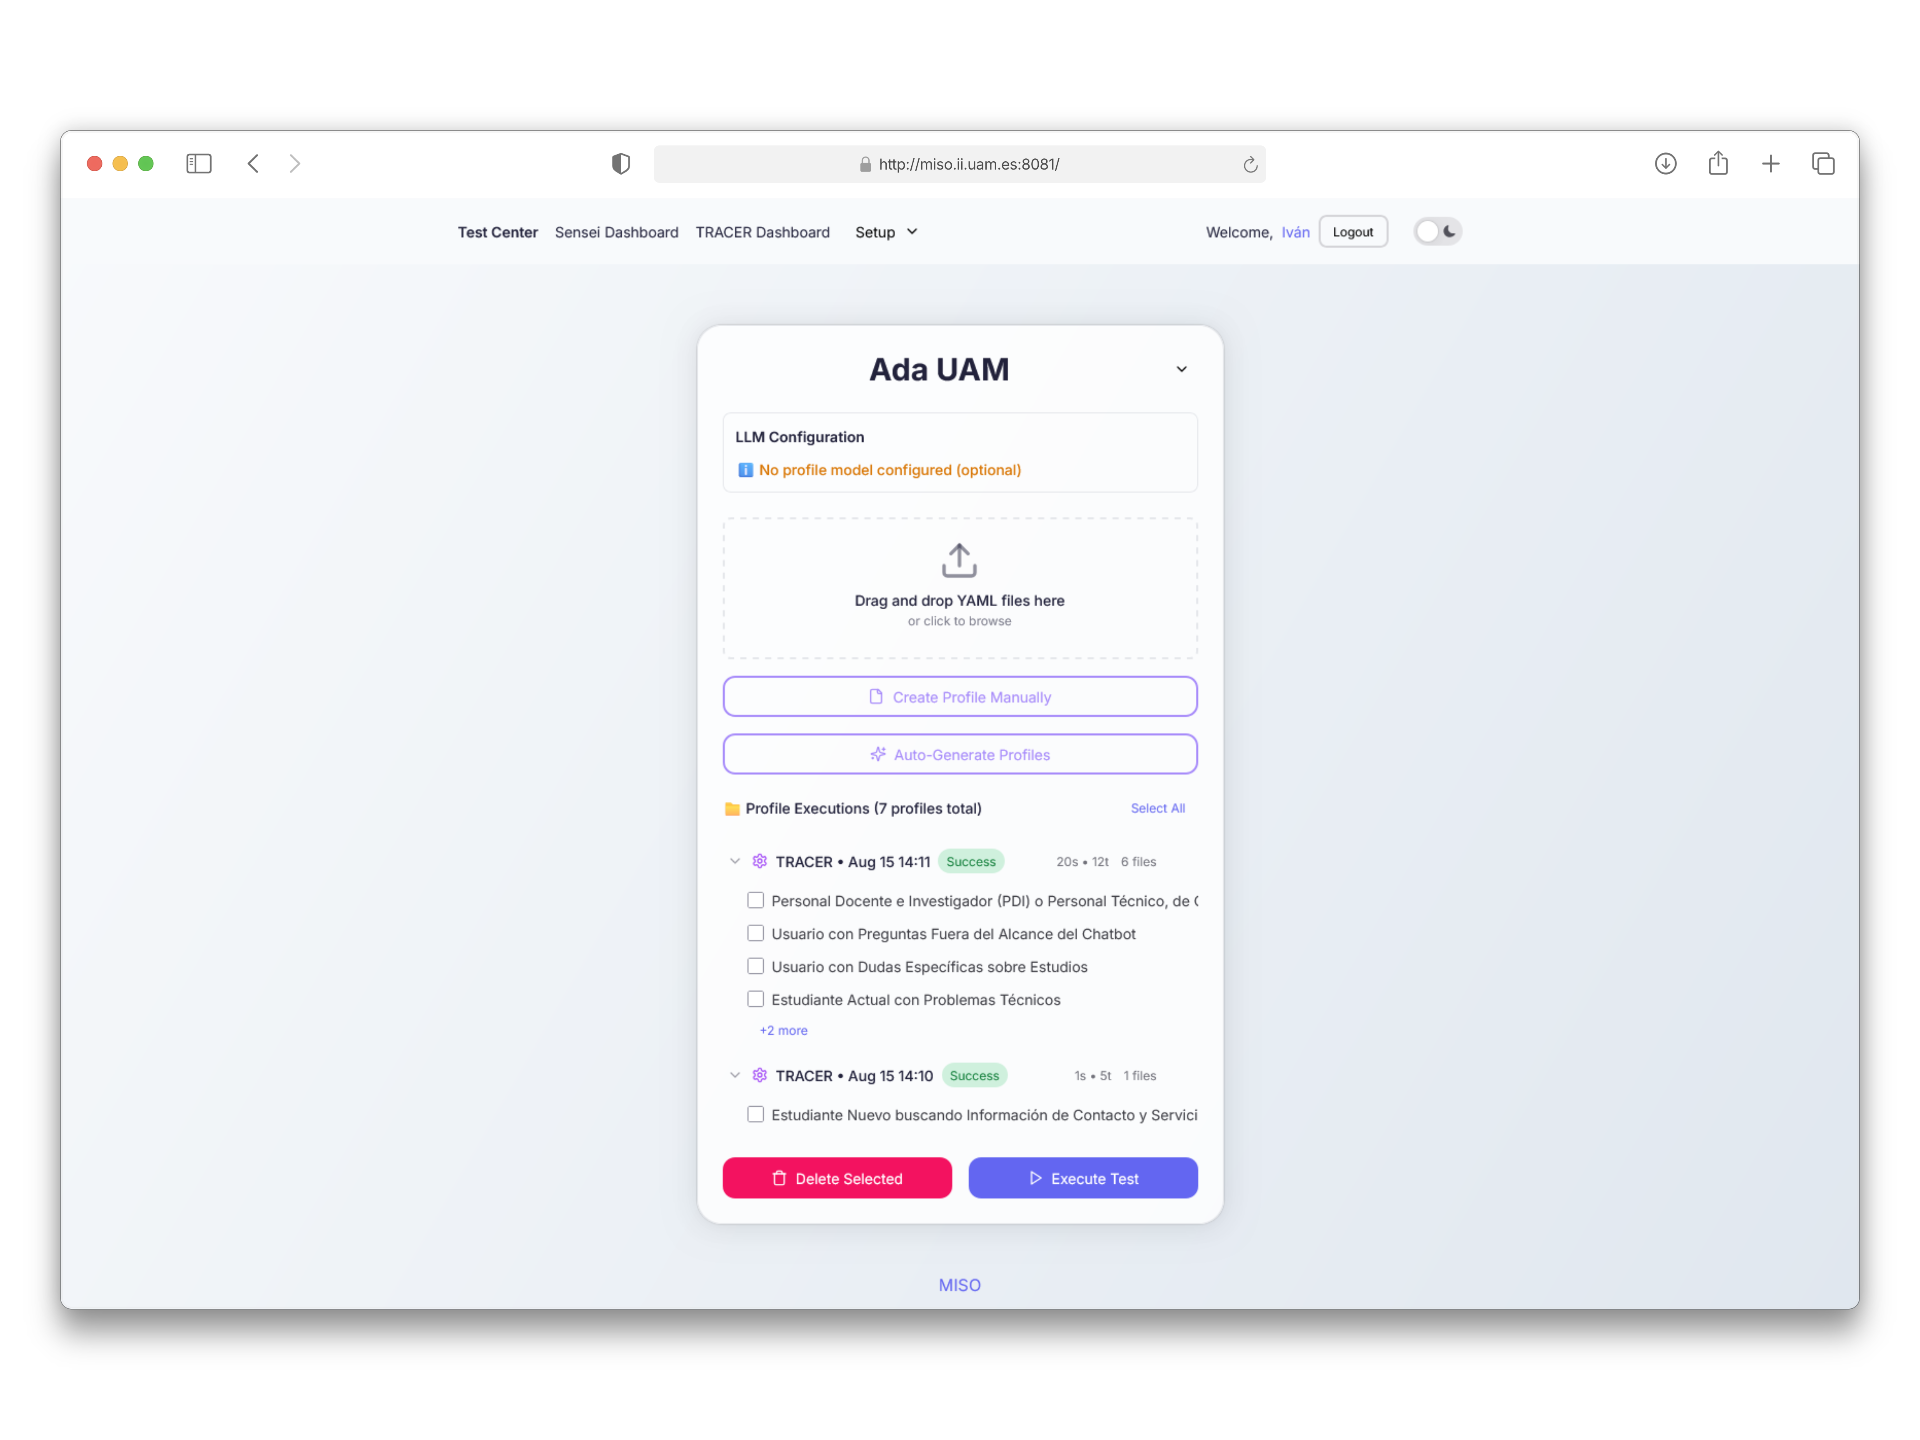
\includegraphics[width=1.1\textwidth]{figures/web-screenshots/test-center-view.png}
  }
  \caption{Screenshot of the test center.}
  \label{fig:ss-test-center}
\end{figure}

After a project is created,
the user can access the test center
(shown in \autoref{fig:ss-test-center}),
this is the main view to managing \ac{TRACER} and SENSEI executions.
Here the user can create and manage the user profiles,
there are two ways to create them:
\begin{itemize}
  \item \textbf{Automated Generation with \ac{TRACER}:}
    the primary method for creating user profiles is employing \ac{TRACER}.
    To do so, the users must click the Auto-Generate Profiles button
    and there choose the number of sessions and turns per session,
    and also the level of verbosity for the logs
    since the user will be able to review them.
    Once the button is clicked, the task is sent to the queue
    and will be executed as soon as possible.
  \item \textbf{Manual Creation:}
    users can also upload their profiles,
    or create them from scratch using an advanced YAML editor.
    This editor contains documentation, autocompletion
    and real-time validation to verify that the YAML syntax is correct
    and that the user profile matches the expected profile schema.
\end{itemize}

With these profiles created,
the users can execute them with SENSEI
by checking the boxes of the profiles they would like to execute
and clicking the \texttt{Execute Test} button.
No further configuration is required.
Once the button is clicked, similar to \ac{TRACER},
the task is sent to the queue.

Once \ac{TRACER} and SENSEI have been executed
the results can be explored in in their respective dashboards.

\begin{figure}[htpb]
  \centering
  \makebox[\textwidth][c]{
      \centering
      \begin{subfigure}{0.52\textwidth}
      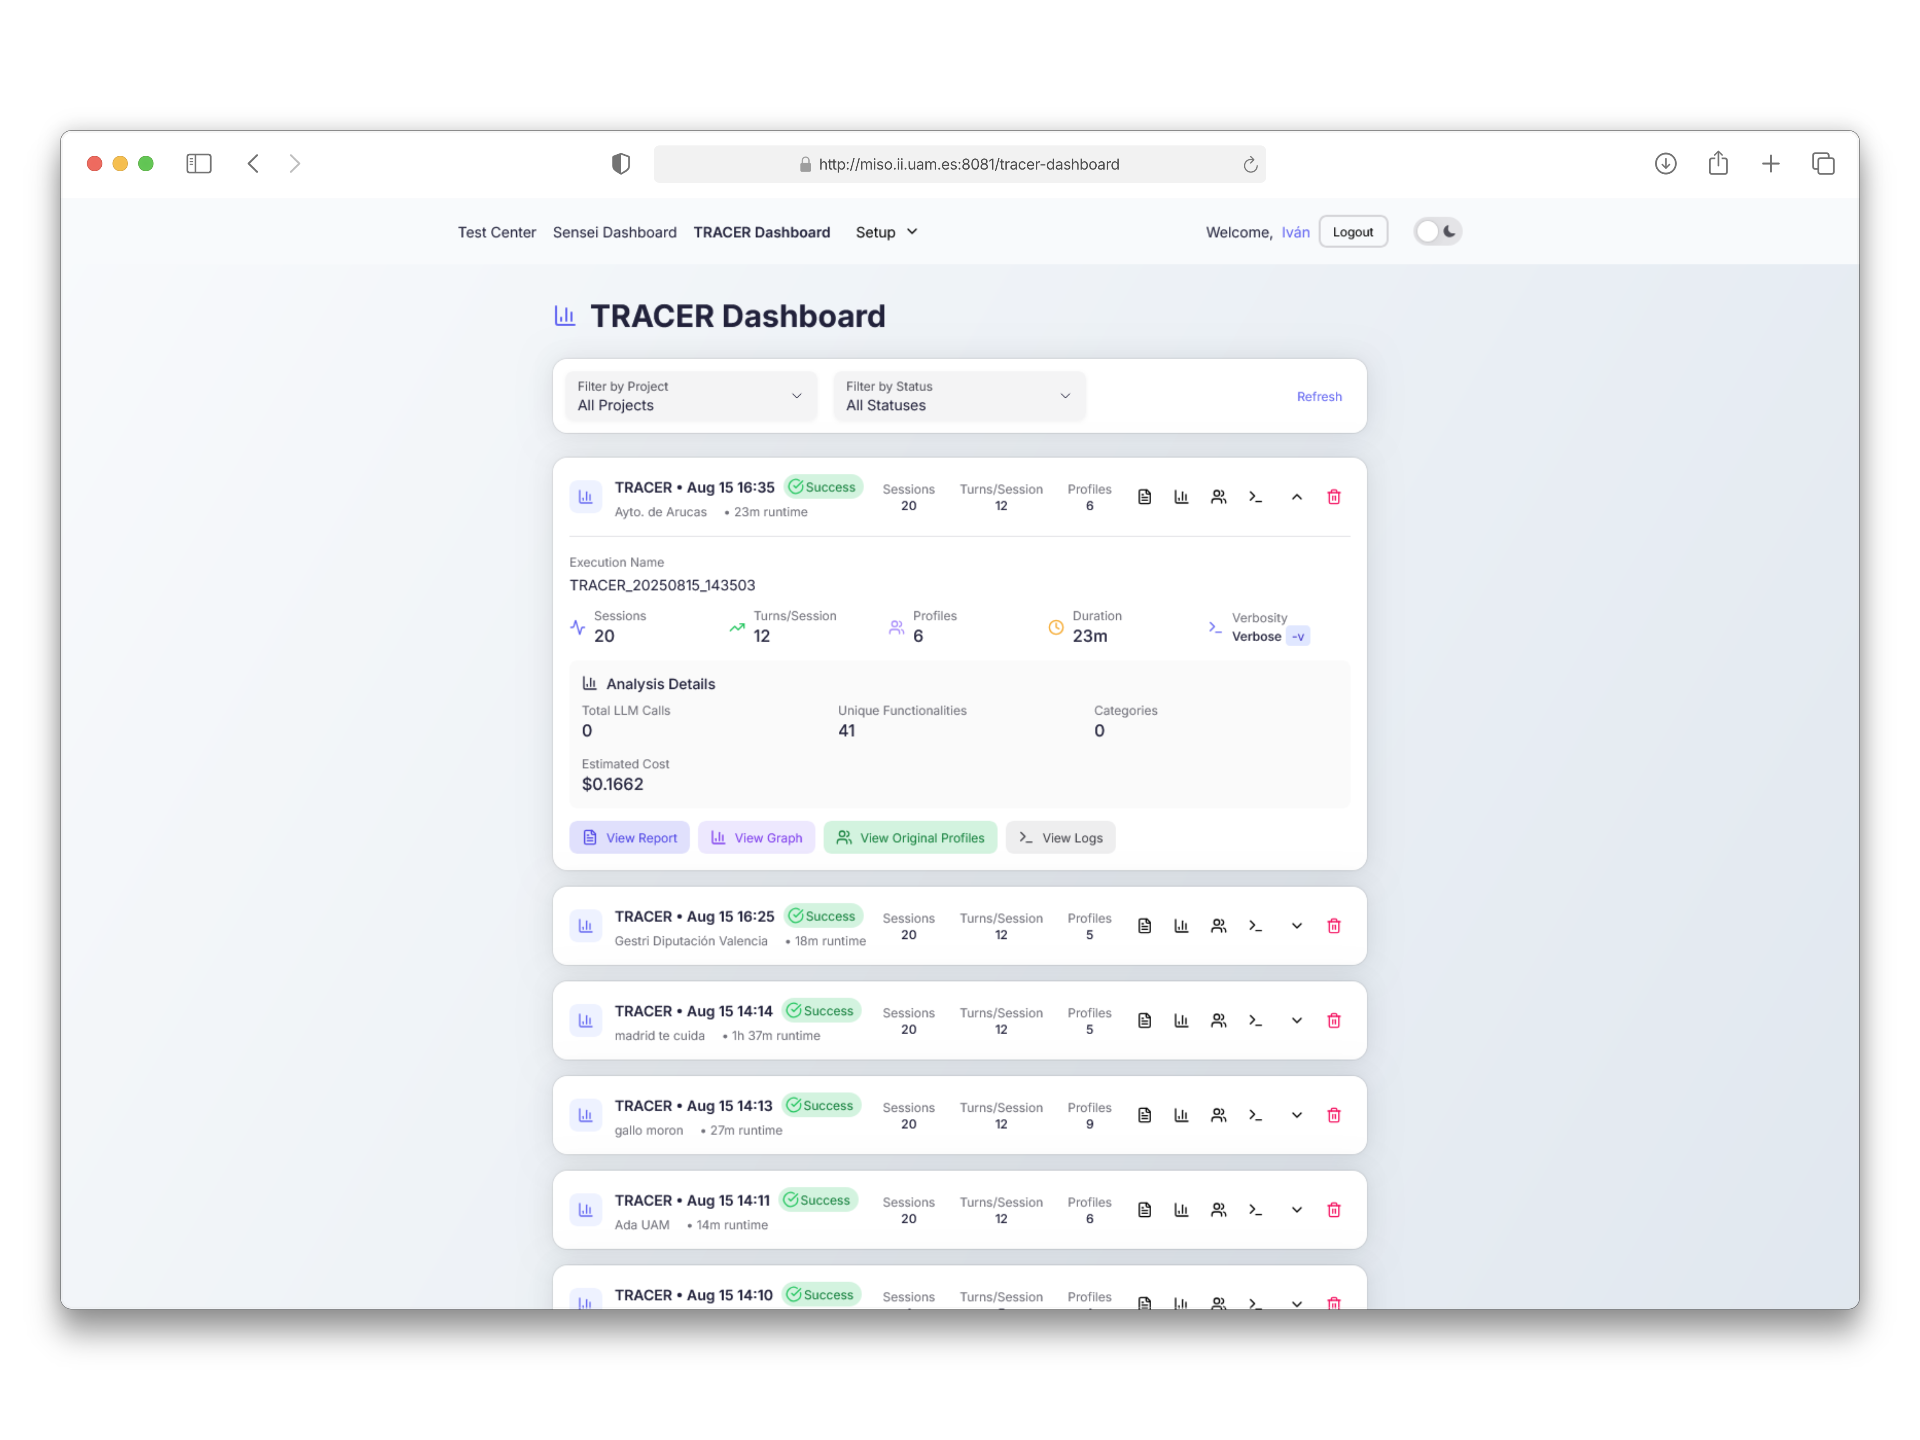
\includegraphics[width=\linewidth]{figures/web-screenshots/tracer-dashboard.png}
      \caption{TRACER dashboard.}
      \label{fig:ss-tracer-dashboard}
    \end{subfigure}
    \begin{subfigure}{0.52\textwidth}
      \centering
      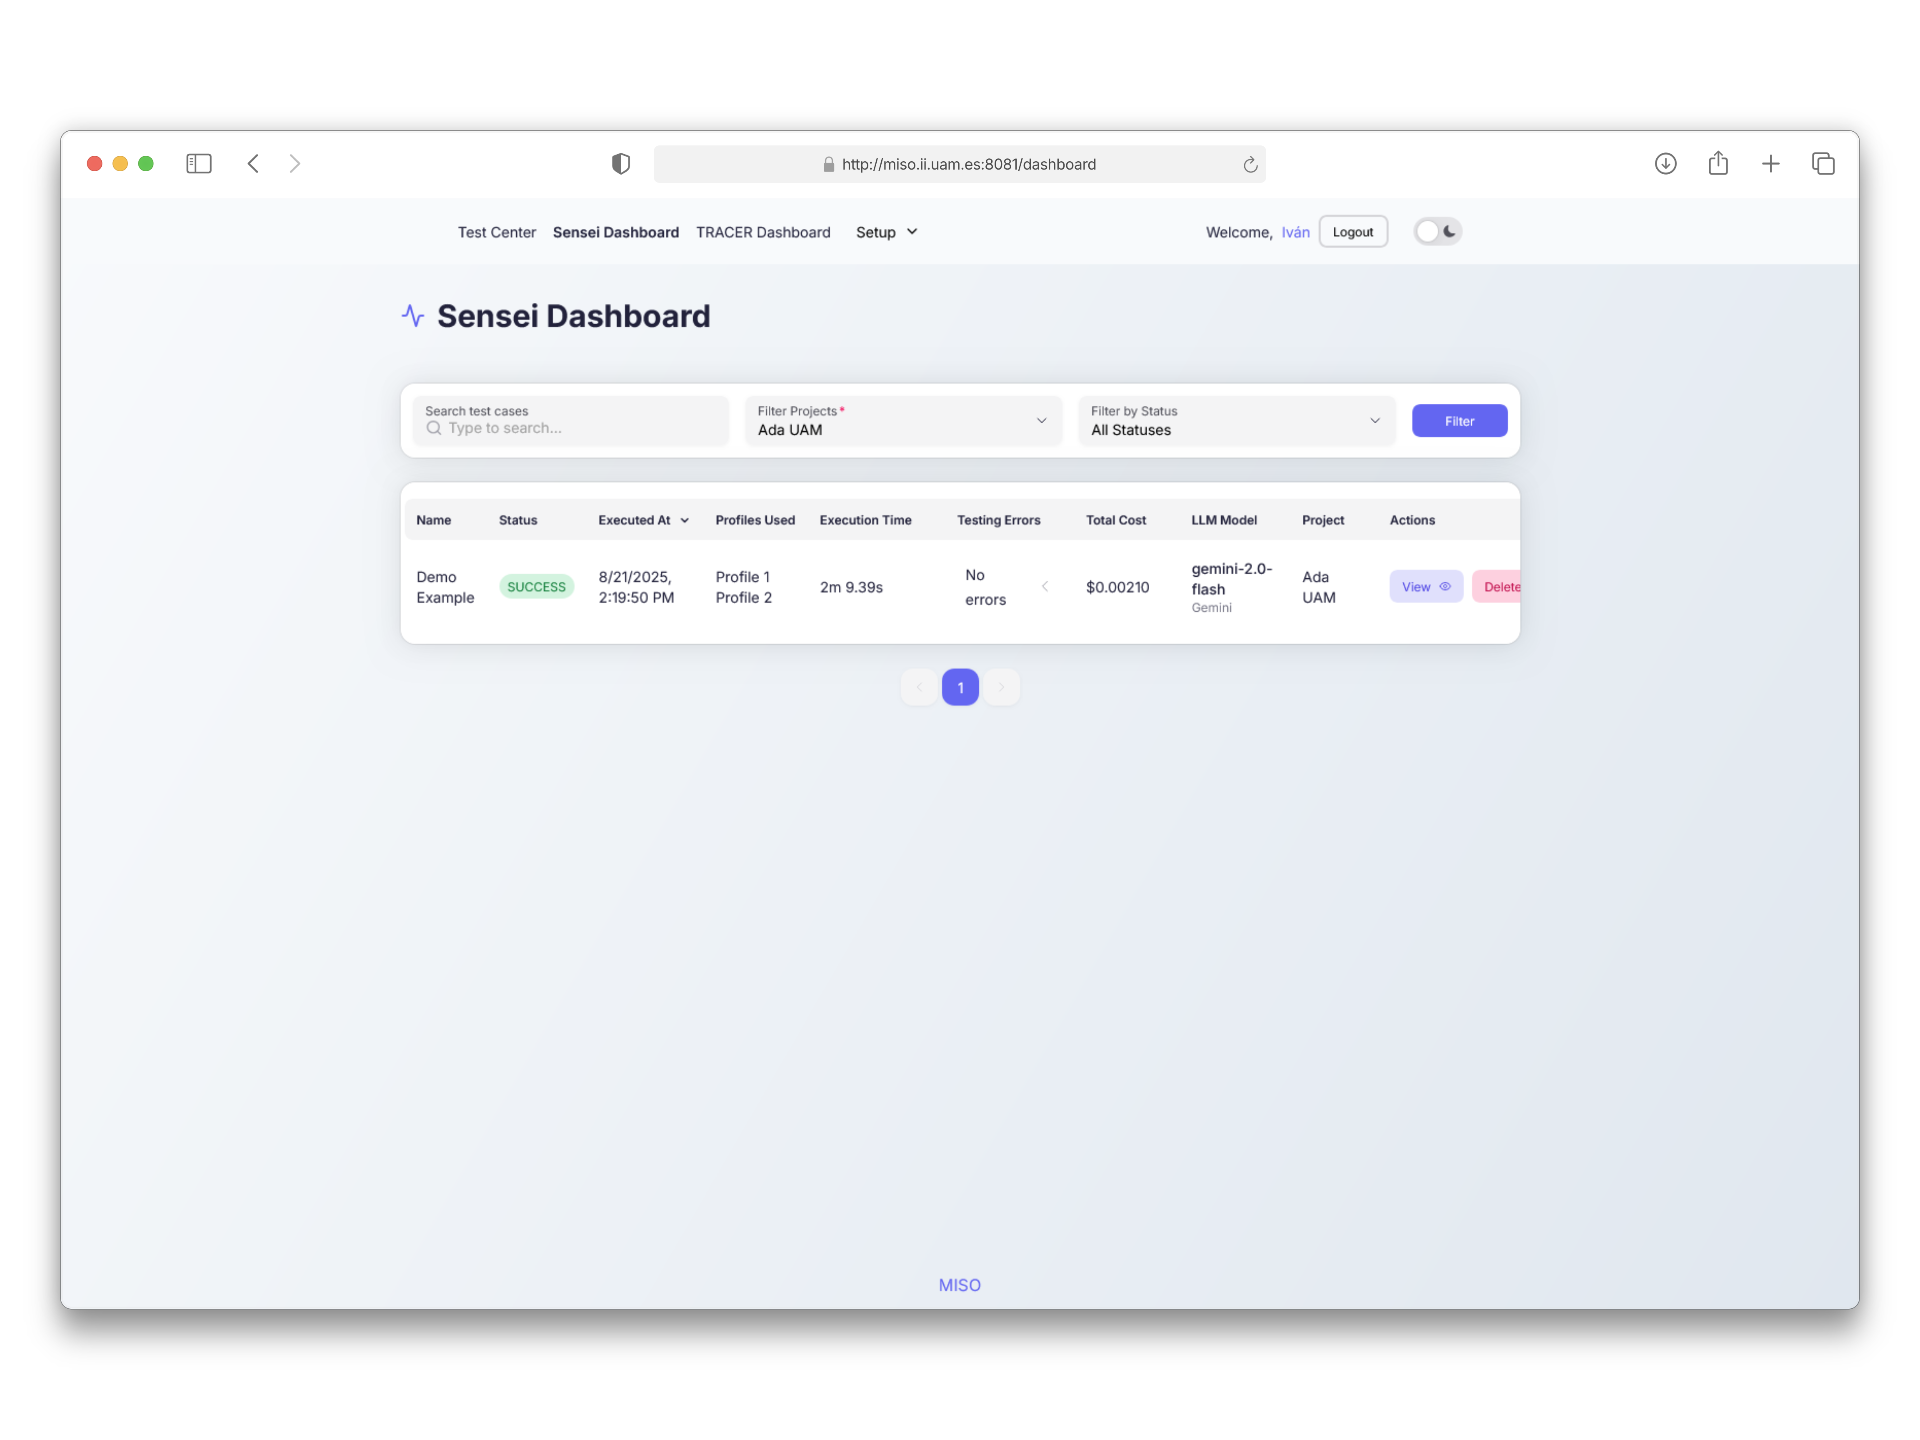
\includegraphics[width=\linewidth]{figures/web-screenshots/sensei-dashboard.png}
      \caption{SENSEI dashboard.}
      \label{fig:ss-sensei-dashboard}
    \end{subfigure}
  }
  \caption{Screenshots of the TRACER and SENSEI dashboards.}
  \label{fig:ss-dashboards}
\end{figure}


The \ac{TRACER} dashboard,
shown in \autoref{fig:ss-tracer-dashboard},
contains a list of the executions
where the users can filter by project and status (running, success, failure, etc.).
Each of these executions has a dropdown arrow to view more information,
the users can also click to see the generated report
containing all the functionalities plus other information in text format,
view the graph where the users can observe the inferred workflow model,
view the original user profiles generated
(note that these are the originals since in the Test Center
the users can modify the profiles to their liking),
and to view the logs, to debug in case of failure, or to read the conversations.



The SENSEI dashboard is shown in \autoref{fig:ss-sensei-dashboard}.
The SENSEI dashboard provides a similar interface
where they can filter SENSEI executions
and then click on one of them to see the results
including the execution times,
errors, cost, and other information.
